\section{Node.js}

\begin{defi}{Node.js}
    \begin{wrapfigure}{r}{0.2\textwidth}
        \centering
        
\includegraphics[width=0.15\textwidth]{includes/figures/defi_node_js.png}
    \end{wrapfigure}
    %
    Neben clientseitigem JavaScript kann man ebenfalls serverseitig dynamisch HTML-Objekte erstellen.
    Viele serverseitige Methoden nutzen die selbe Syntax wie clientseitige Methoden.

    \emph{Node.js} ist ein eventbasierter Webserver.

    Bei einer Anfrage wird ein Thread erstellt, welcher genutzt wird, um diese synchron abzuarbeiten.

    Der Haupt-Thread wird dabei jedoch nicht blockiert.
    Jeder Worker-Thread läuft dabei in einer eigenen JavaScript Engine.

    Ein erster Ansatz sieht wie folgt aus\footnote{Node.js erstellt einen Worker-Thread (hier blau)}:
    \begin{center}
        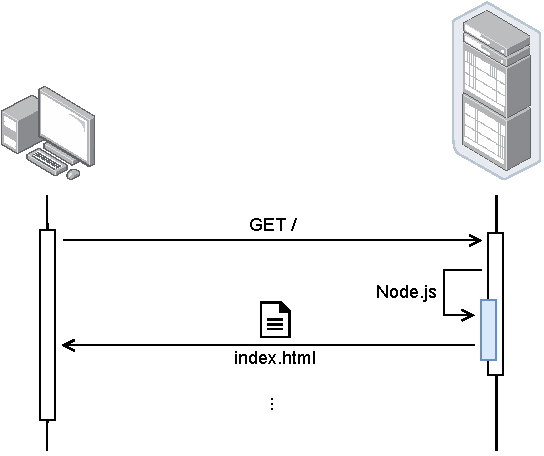
\includegraphics[width=0.5\textwidth]{includes/figures/defi_js_server.pdf}
    \end{center}
    Auf dem Server existiert potentiell keine Datei \texttt{index.html}, sondern wird immer neu erstellt.
\end{defi}

\begin{example}{Ordnerstruktur}
    \begin{center}
        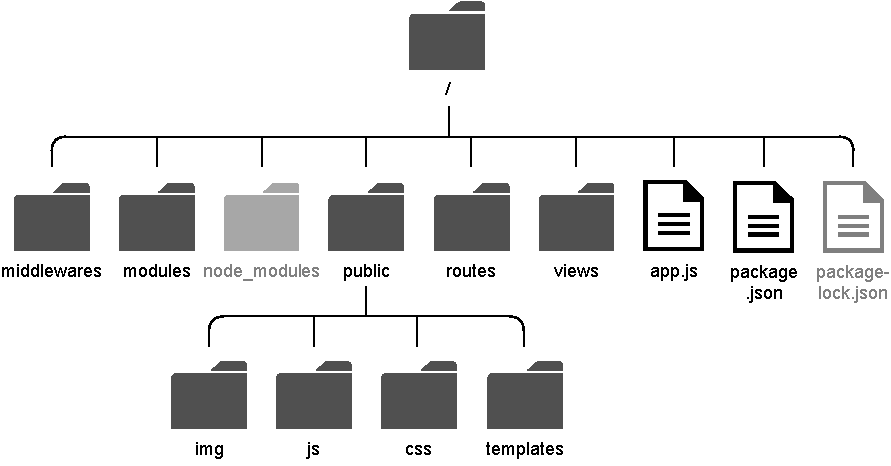
\includegraphics[width=0.75\textwidth]{includes/figures/example_nodejs_ordnerstruktur.pdf}
    \end{center}
\end{example}

\subsection{Projekt}

\begin{center}
    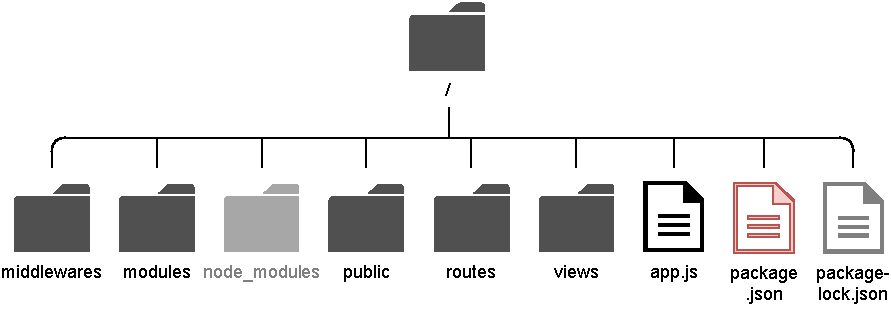
\includegraphics[width=0.75\textwidth]{includes/figures/bonus_nodejs_package.pdf}
\end{center}

\begin{defi}{package.json}
    \texttt{npm init} erzeugt interaktiv eine \texttt{package.json}, welche Informationen über das Node-Projekt (wie z. B. Abhängigkeiten) enthält.

    Enthält der Ordner diese \texttt{package.json}, wird sie von Node als Projekt erkannt und kann mit \texttt{node .} ausgeführt werden.
\end{defi}

\subsection{Module}

\begin{defi}{Modul}
    Ein \emph{Modul} ist eine Funktionalität, die in eine eigene JavaScript-Datei ausgelagert wurde.

    Man unterteilt JavaScript-Module in drei Arten:
    \begin{enumerate}
        \item \emph{Integrierte Module}:
              \begin{itemize}
                  \item Vorinstallierte Kernmodule
              \end{itemize}
        \item \emph{Lokale Module}:
              \begin{itemize}
                  \item Meist selbstgeschriebene Funktionen und Klassen
                  \item Zu finden in \texttt{/modules}
              \end{itemize}
        \item \emph{Third-Party-Module}:
              \begin{itemize}
                  \item Öffentliche Module, welche per Package Manager (\texttt{npm}) eingebunden werden
                  \item Zu finden in \texttt{/node\_modules}
              \end{itemize}
    \end{enumerate}

    Zum Nutzen der Module muss man in einer JavaScript-Datei folgende Import-Anweisung nutzen:
    \begin{lstlisting}[language=JavaScript]
        const MODULE = require('/modules/file.js')
    \end{lstlisting}
\end{defi}

\begin{center}
    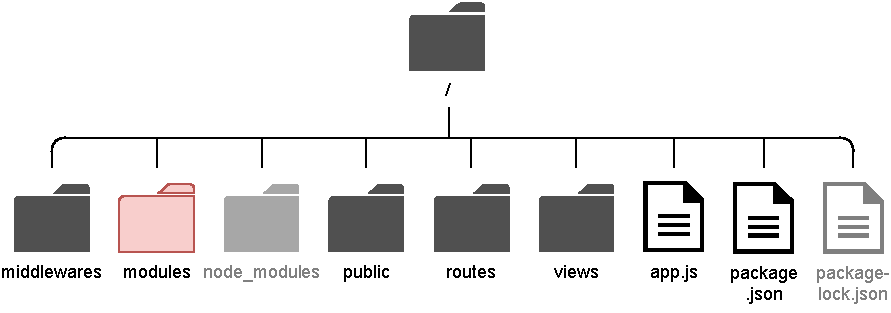
\includegraphics[width=0.75\textwidth]{includes/figures/bonus_nodejs_module.pdf}
\end{center}

\begin{defi}{Modulexport}
    Zum \emph{Exportieren} einer Funktion muss man nach der Initialisierung der Methode bzw. Klasse folgendes Export-Anweisung nutzen:
    \begin{lstlisting}[language=JavaScript]
        module.exports = ...
    \end{lstlisting}
\end{defi}

\begin{example}{Modulexport (einfach)}
    Um \emph{Klassen} direkt zu exportieren, überschreibt man \texttt{module.exports}:

    \texttt{modules/pokemon.js}
    \begin{lstlisting}[language=JavaScript]
        ^class Pokemon^ {
            id, name

            constructor(id, name) {
                this.id = id,
                this.name = name
            }

            toString() {
                return `${this.name} [${this.id}]`
            }
        }

        module.exports = ^Pokemon^
    \end{lstlisting}

    \texttt{app.js}
    \begin{lstlisting}[language=JavaScript]
        const ^Pokemon^ = require('modules/pokemon.js')

        const glumanda = ^new Pokemon(4, 'Glumanda')^
        console.log(glumanda.toString()) // Glumanda [4]
    \end{lstlisting}

    Alternativ kann man direkt \emph{Instanzen} exportieren (z. B. für Singleton etc.):

    \texttt{modules/pokemon.js}
    \begin{lstlisting}[language=JavaScript]
        class Pokemon { ... }

        module.exports = ^new Pokemon(4, 'Glumanda')^
    \end{lstlisting}

    \texttt{app.js}
    \begin{lstlisting}[language=JavaScript]
        const ^glumanda^ = require('modules/pokemon.js')

        console.log(glumanda.to_string()) // Glumanda [4]
    \end{lstlisting}
\end{example}

\begin{example}{Modulexport (mehrfach)}
    Um mehrere Objekte zu exportieren, kann man entweder \texttt{module.exports}\footnote{
        Wenn man nur das Objekt anpasst, kann man \texttt{exports = ...} nutzen, da \texttt{exports} ein pointer auf \texttt{module.exports} ist.
        Beim Überschreiben der Variable wird nur die Referenz auf \texttt{module.exports} gelöscht.
    } anpassen:

    \texttt{modules/pokemon.js}
    \begin{lstlisting}[language=JavaScript]
        class Pokemon { ... }
        class Attacke { ... }
        function brennen(p) { ... }

        /* module. */ exports.Pokemon = Pokemon
        /* module. */ exports.Attacke = Attacke
        /* module. */ exports.brennen = brennen
    \end{lstlisting}

    \texttt{app.js}
    \begin{lstlisting}[language=JavaScript]
        const pokemon_module = require('modules/pokemon.js')

        pokemon_module.brennen(new pokemon_module.Pokemon(4, 'Glumanda'))
    \end{lstlisting}

    oder mit einem Array überschreiben:

    \texttt{modules/pokemon.js}
    \begin{lstlisting}[language=JavaScript]
        class Pokemon { ... }
        class Attacke { ... }
        function brennen(p) { ... }

        module.exports = [Pokemon, Attacke, brennen]
    \end{lstlisting}

    \texttt{app.js}
    \begin{lstlisting}[language=JavaScript]
        const [Pokemon, Attacke, brennen] = require('modules/pokemon.js')

        brennen(new Pokemon(4, 'Glumanda'))
    \end{lstlisting}

    Man sieht, dass man in der ersten Variante deutlich mehr schreiben muss, da man den \enquote{namespace} vor jedes Objekt des Modules schreiben muss.
    Jedoch hat sie den deutlichen Vorteil, dass man nicht alle imports anpassen muss, wenn man einen export hinzufügt.
\end{example}

\subsection{Öffentliche Module}

\begin{defi}{Node Package Manager}
    \emph{Node Package Manager (npm)} ist ein Projektmanager für Node.js.
    Er wird genutzt um Öffentliche Module zu importieren oder eigene Module öffentlich zur Verfügung zu stellen.
\end{defi}

\begin{center}
    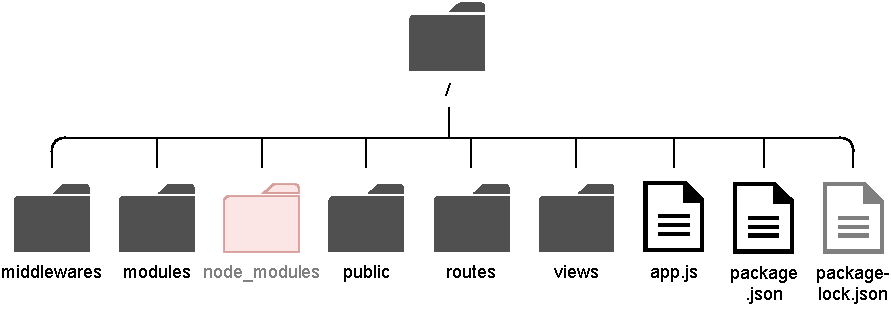
\includegraphics[width=0.75\textwidth]{includes/figures/bonus_nodejs_node_modules.pdf}
\end{center}

\begin{bonus}{node\_modules}

    Um ein öffentliches Modul einer \texttt{package.json} hinzuzufügen und dieses direkt zu laden, nutzt man:

    \begin{center}
        \texttt{npm install <package>}
    \end{center}

    Wenn eine fremde \texttt{package.json} eingebunden hat und alle Module laden möchte, von denen das Projekt abhängig ist, nutzt man:
    \begin{center}
        \texttt{npm install}
    \end{center}

    Einige relevante Module sind:
    \begin{itemize}
        \item \emph{Mustache}, zum Rendern von HTML-Templates
        \item \emph{Sequelize}, für den Zugriff auf eine Datenbank
    \end{itemize}
\end{bonus}

\subsubsection{Websockets}

\begin{defi}{Websocket}
    \emph{Websockets} ermöglichen Kommunikation mittels bestimmter Kommunikationsprotokolle.

    Generell kann man unterscheiden zwischen:
    \begin{itemize}
        \item \emph{Stream-Sockets}:
              \begin{itemize}
                  \item kommunizieren über einen Zeichen-Datenstrom
                  \item verwenden meist TCP
              \end{itemize}
        \item \emph{Datagramm-Sockets}:
              \begin{itemize}
                  \item kommunizieren über einzelne Nachrichten
                  \item verwenden meist UDP
              \end{itemize}
    \end{itemize}
\end{defi}

\begin{example}{Websocket}
    \texttt{app.js}:
    \begin{lstlisting}[language=JavaScript]
        const express = require('express')
        const app = express()

        const port = 3000

        app.use('/', express.static(__dirname + '/public')))

        const server = app.listen(port)

        const ws = new require('ws').Server({ server }) // alternativ 'noServer: true'
        ws.on('connection', require('./modules/connection.js'))
    \end{lstlisting}

    \texttt{modules/connection.js}
    \begin{lstlisting}[language=JavaScript]
        module.exports = (socket, req) =>
            socket.on('message', massage => socket.send('GGAAWWRRR'))
    \end{lstlisting}

    \texttt{public/index.html}:
    \begin{lstlisting}[language=HTML5]
        <!DOCTYPE html>
        <html>
        <head>
            <title>Pokemon</title>
            <script src="/js/ws.js"></script>
        </head>

        <body> <button id="btn_talk">talk</button> </body>
        </html>
    \end{lstlisting}

    \texttt{public/js/ws.js}
    \begin{lstlisting}[language=JavaScript]
        let socket = new WebSocket('wss://localhost:3000/') // wss = web socket secure
        socket.onopen = () => console.log('CLIENT: connected')
        socket.onmessage = message => console.log(`CLIENT: ${message.data}`)

        window.onload = () =>
            document.getElementById('btn_talk').addEventListener('click', event =>
                socket.send('Mache ein Geraeusch')
            )
    \end{lstlisting}
\end{example}

\subsection{Einstiegspunkt}

\begin{center}
    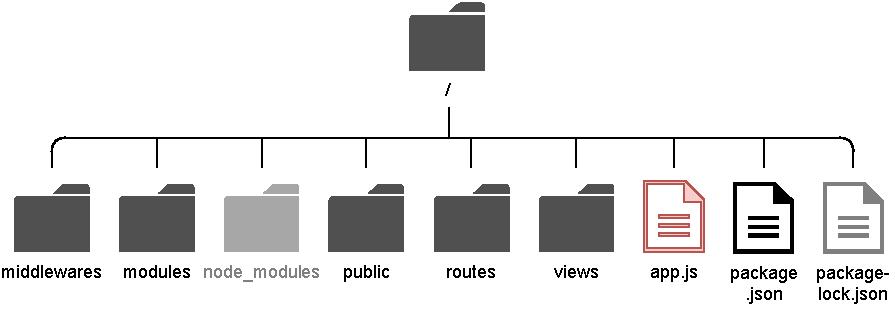
\includegraphics[width=0.75\textwidth]{includes/figures/bonus_nodejs_app.pdf}
\end{center}

\begin{bonus}{app.js}
    Die \texttt{app.js} ist der standardmäßige Einstiegspunkt einer Node-Anwendung.

    In der \texttt{package.json} wird festgelegt, welche Datei diese Aufgabe übernimmt.

    Der Server wird mit \texttt{node .} gestartet.
\end{bonus}

\begin{example}{app.js}
    Ein reiner Webserver kann wie folgt erstellt werden; es wird ausschließlich das vorinstallierte Modul \texttt{http} benötigt:

    \begin{lstlisting}[language=JavaScript]
        const http = require('http')

        const port = 3000

        function handleRequest(req, res) {
            res.end(req.url + ': hello')
        }

        const server = http.createServer(handleRequest)
        server.listen(port)
    \end{lstlisting}

    Wenn man nun die URL \texttt{http://localhost:3000/test} aufruft, erhält man:
    \begin{center}
        \texttt{/test: hello}
    \end{center}
\end{example}

\begin{defi}{Express}
    \emph{Express} ist das meistgenutzte Web-Framework für Node.js.

    Es erweitert Node.js um Werkzeuge, mit denen das Entwickeln moderner Webanwendungen einfacher gestaltet wird.
\end{defi}

\begin{example}{app.js (Express)}
    \begin{lstlisting}[language=JavaScript]
        const express = require('express')
        
        const app = express()
        const port = 3000

        app.get('/', (req, res) => {
            res.send('hello')
        })

        app.listen(port)
    \end{lstlisting}

    Wenn man nun die Webseite \texttt{http://localhost:3000/} aufruft, erhält man:
    \begin{center}
        \texttt{hello}
    \end{center}

    Die Routen werden jedoch meist nicht in der \texttt{app.js} definiert, sondern lediglich eingebunden:
    \begin{lstlisting}[language=JavaScript]
        app.use(require('routes/file.js'))
    \end{lstlisting}
\end{example}

\subsection{Routen}

\begin{center}
    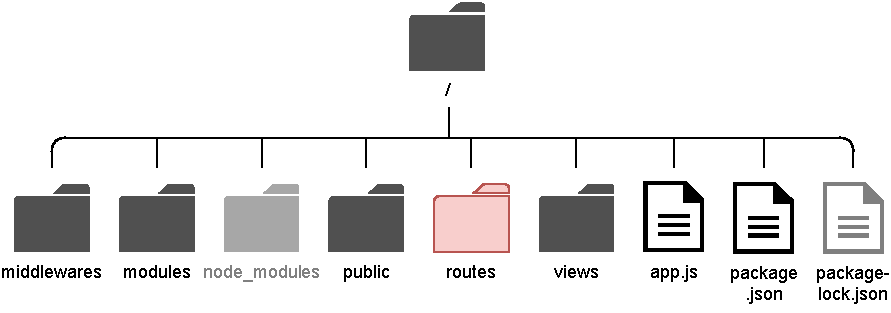
\includegraphics[width=0.75\textwidth]{includes/figures/bonus_nodejs_routes.pdf}
\end{center}

\begin{defi}{Route}
    \emph{Routen} dienen zur Navigation innerhalb einer Anwendung.

    Sie werden als Callback-Methode abgebildet:

    \begin{center}
        \texttt{.get('/'. (req, res, next) => {})}
    \end{center}

    Die Syntax besteht aus folgenden Teilen:
    \begin{itemize}
        \item \emph{HTTP-Methode}:
              \begin{itemize}
                  \item z. B. \texttt{get}, \texttt{post}, \texttt{put}, \texttt{patch}, \texttt{delete} etc.
                  \item \texttt{all}: Alle \emph{HTTP Methoden}
                  \item \texttt{use}: Alle \emph{HTTP Methoden}, inkl. rekursiv aller Subrouten
              \end{itemize}
        \item \emph{Path}:
              \begin{itemize}
                  \item Route, die im Browser genutzt wird. z. B. \texttt{/}
                  \item Mögliche Eingaben: String, Muster, Regex, Array
              \end{itemize}
        \item \texttt{req}:
              \begin{itemize}
                  \item \emph{HTTP Request Argument} mit übergebenen Parametern
              \end{itemize}
        \item \texttt{res}:
              \begin{itemize}
                  \item \emph{HTTP Response Argument}, die hier erstellt wird
                  \item Beispiele:
                        \begin{itemize}
                            \item \texttt{res.download()} (fordert Client auf, eine Datei herunterzuladen)
                            \item \texttt{res.end()} (beendet den Prozess)
                            \item \texttt{res.json()} (sendet JSON-Objekt)
                            \item \texttt{res.redirect()} (leitet Client weiter)
                            \item \texttt{res.render()} (rendert Anzeigevorlage)
                            \item \texttt{res.send()} (sendet Antwort mit beliebigem Typen)
                            \item \texttt{res.sendFile()} (sendet Datei als Oktett-Stream)
                            \item \texttt{res.sendStatus()} (legt Antwortstatuscode fest)
                        \end{itemize}
              \end{itemize}
        \item \texttt{next}:
              \begin{itemize}
                  \item Callback-Methode die ausgeführt werden muss, sollten weitere Routen existieren, die unter dem Pfad liegen.
                  \item \texttt{next()} wird in Middlewares genutzt.
              \end{itemize}
    \end{itemize}
\end{defi}

\begin{defi}{Router}
    Wenn man mehrere Routen bündeln möchte, nutzt man \emph{Router}.

    Man schafft eine Hierarchie um Unterpfade getrennt von den Routern zur Verfügung zu stellen und die Routennamen, falls nötig, zu parametrisieren.

    So wird z. B. aus:
    \begin{lstlisting}[language=JavaScript]
        app.get(^'/base_route/a'^, (req, res) => { ... })
        app.get(^'/base_route/b'^, (req, res) => { ... })
        app.get(^'/base_route/c'^, (req, res) => { ... })
    \end{lstlisting}

    direkt:
    \begin{lstlisting}[language=JavaScript]
        const router = express.Router()
        
        router.get('/a', (req, res) => { ... })
        router.get('/b', (req, res) => { ... })
        router.get('/c', (req, res) => { ... })
        
        app.use(^'base_route'^, router)
    \end{lstlisting}

    Eine Ansammlung von Routern findet man im Ordner \texttt{/routes}.
\end{defi}

\begin{example}{Router}
    \texttt{app.js}:
    \begin{lstlisting}[language=JavaScript]
        const express = require('express')
        const app = express()

        /* routes */
        app.use(^'/pokemon'^, require('routes/pokemon.js'))

        app.listen(3000)
    \end{lstlisting}

    \texttt{routes/pokemon.js}:
    \begin{lstlisting}[language=JavaScript]
        const Pokemon = require('../modules/pokemon.js') // definiert Pokemon-Klasse
        const express = require('express')
        
        module.exports = express.Router()
            .get(^'/'^, (req, res) => {
                res.send(Pokemon.getRand().toString())
            })
            .get(^'/count'^, (req, res) => {
                res.send('896')
            })
    \end{lstlisting}

    Wenn man nun die Webseite \texttt{http://localhost:3000/pokemon} aufruft, erhält man z. B.:

    \begin{center}
        \texttt{Glumanda [4]}
    \end{center}

    Wenn man die Webseite \texttt{http://localhost:3000/pokemon/count} aufruft, erhält man:

    \begin{center}
        \texttt{896}
    \end{center}
\end{example}

\begin{defi}{Validierung (JavaScript)}
    Beschränkungen auf Clientseite können von erfahrenen Nutzenden aktiv umgangen werden, daher ist eine serverseitige Prüfung von Userdaten zwingend erforderlich.

    \texttt{express-validator} vereinfacht in JavaScript die Validierung von Eingaben.

    Sie liefern \texttt{NULL}, \texttt{false} oder eine je nach Filter gültige Variable zurück.

    \begin{itemize}
        \item \texttt{Validators} validieren Eingaben
        \item \texttt{Sanitizers} korrigieren Eingaben
    \end{itemize}

    Validator:
    \begin{lstlisting}[language=JavaScript]
        const { check } = require('express-validator')

        app.use('/pokemon', [                      // check pokemon
            check('pokemon').isLength({ min: 3 }), // min. length 3 chars (z. B. Mew)
        ])
    \end{lstlisting}

    Sanitizer:
    \begin{lstlisting}[language=JavaScript]
        const { check } = require('express-validator')

        app.use('/pokemon', [         // check pokemon
            check('id').toInt()       // parse ID to Int
            check('Pokemon').escape() // '<Glumanda%>' -> '&lt;Glumanda%&gt;'
        ])
    \end{lstlisting}
\end{defi}

\subsubsection{REST}

\begin{defi}{REST}
    \emph{REpresentational State Transfer (REST)} dient als Architektur unter dem HTTP-Transportprotokoll, um mit Ressourcen zu interagieren.

    REST ist zustandslos.
    Der Server behandelt jeden Aufruf als in sich abgeschlossenen Auftrag ohne impliziten Bezug auf vorgehende Operationen.
\end{defi}

\begin{defi}{Hypermedia}
    \emph{Hypermedia} bezeichnet Medien, die (untereinander) mithilfe von Hyperlinks vernetzt sind.

    Hypermedia kann sich aus allen Typen und Formen von Medien zusammensetzen.
\end{defi}

\begin{defi}{CRUD}
    Alle REST-Interaktionen lassen sich mittels einfacher Abbildungen auf die HTTP-Verben beschreiben.

    Dazu nutzen wir die bekannten \emph{CRUD (Create, Read, Update, Delete)}-Operationen.
\end{defi}

\begin{example}{GET (REST)}
    \begin{center}
        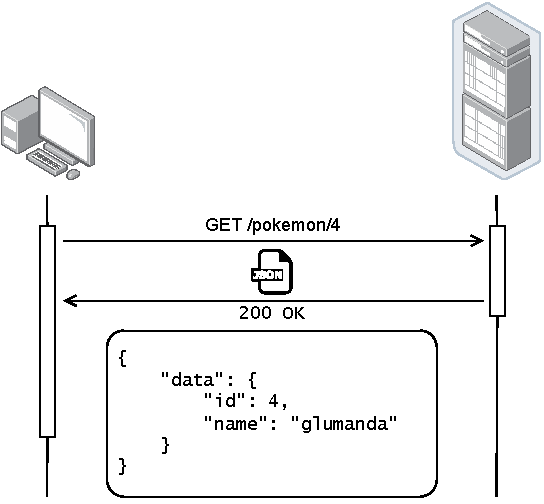
\includegraphics[width=0.5\textwidth]{includes/figures/example_rest_get.pdf}
    \end{center}
\end{example}

\begin{example}{POST (REST)}
    \begin{center}
        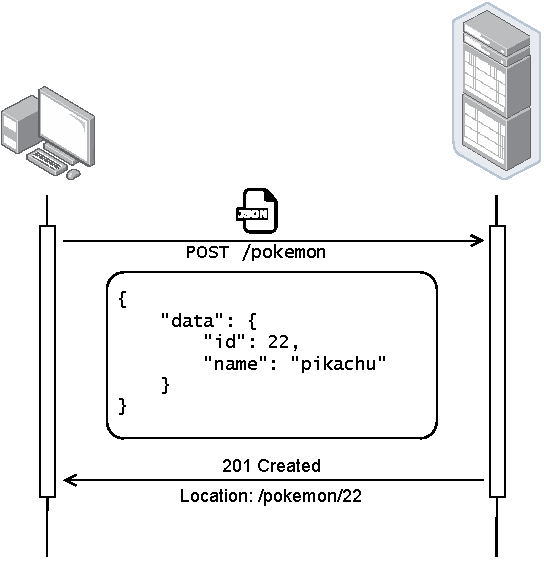
\includegraphics[width=0.5\textwidth]{includes/figures/example_rest_post.pdf}
    \end{center}
\end{example}

\begin{bonus}{Rückgabetypen}
    In Express-Routen ist es bei einer REST-Schnittstelle sinnvoll, anstatt \texttt{res.send()} in einem Switch für das Format, \texttt{res.format()} zu nutzen.

    Dadurch kann man sinnvoll auf das gewünschte Format des Clients reagieren:

    \begin{lstlisting}[language=JavaScript]
        res.format({
            text: () => res.send('Glumanda [4]')
            html: () => res.send('<p> Glumanda [4] </p>')
            json: () => res.send({ 'id': 4, 'name': 'Glumanda'})
        })
    \end{lstlisting}
\end{bonus}

\begin{bonus}{Parameterübergabe}
    \begin{itemize}
        \item Wiederholung: \texttt{GET}:

              \begin{lstlisting}[language=JavaScript]
                  // URL z. B.: https://paddel.xyz/pokemon?id=4&name=Glumanda
                  module.exports = express.Router()
                      .^get^('/', (req, res) => {
                          console.log(req.^query^) // { 'id': 4, 'name': 'Glumanda' }
                      })
              \end{lstlisting}
        \item Wiederholung: \texttt{POST}:

              \begin{lstlisting}[language=JavaScript]
                // reminder: bodyParser
                module.exports = express.Router()
                    .^post^('/', (req, res) => {
                        console.log(req.^body^) // { 'id': 4, 'name': 'Glumanda' }
                    })
            \end{lstlisting}
        \item \texttt{params}:

              \begin{lstlisting}[language=JavaScript]
                module.exports = express.Router()
                    .get(^'/:id/:name'^, (req, res) => {
                        console.log(req.^params^) // { 'id': 4, 'name': 'Glumanda' }
                    })
            \end{lstlisting}
    \end{itemize}
\end{bonus}

\subsection{Middlewares}

\begin{center}
    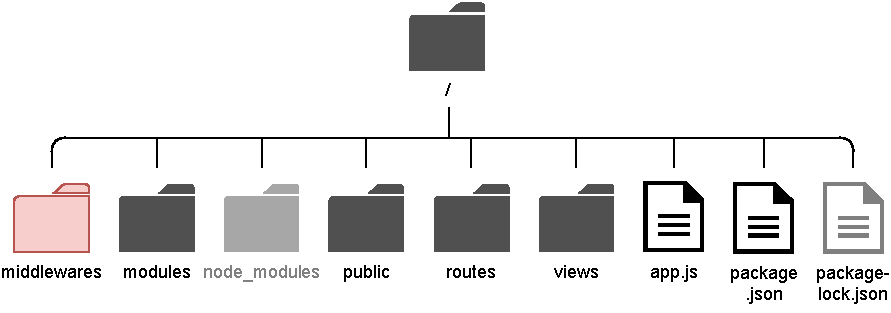
\includegraphics[width=0.75\textwidth]{includes/figures/bonus_nodejs_middlewares.pdf}
\end{center}

\begin{defi}{Middleware}
    \emph{Middlewares} sind ein Stack von Funktionen mit beliebigem Inhalt.

    Sie werden zwischen dem Eingehen eines Requests und dessen Bearbeitung durch eine Handlerfunktion geschaltet.

    In Middlewares können z. B. Eingaben geparsed werden, geloggt werden oder Fehler abgefangen werden.\footnote{Anmeldungen werden ebenfalls über Middlewares geregelt.}

    Sie haben Zugriff auf \emph{Request}, \emph{Response}, sowie den direkt folgende \emph{Middleware-Callback}.
\end{defi}

\begin{example}{Middleware}
    \texttt{app.js}:
    \begin{lstlisting}[language=JavaScript]
        const express = require('express')
        const app = express()

        /* middlewares */ app.use(^'/'^, require('middlewares/logging.js')) // 1.
        /* routes */ app.use(^'/pokemon'^, require('routes/pokemon.js')) // 2.

        app.listen(3000)
    \end{lstlisting}

    \texttt{routes/pokemon.js}:
    \begin{lstlisting}[language=JavaScript]
        const Pokemon = require('../modules/pokemon.js') // definiert Pokemon-Klasse
        const express = require('express')
        
        module.exports = express.Router()
            .get(^'/'^, (req, res) => res.send(Pokemon.getRand().toString()) )
    \end{lstlisting}

    \texttt{middlewares/logging.js}:
    \begin{lstlisting}[language=JavaScript]
        const express = require('express')
        
        module.exports = express.Router()
            .get(^'/*'^, (req, res, next()) => {
                console.log(req.url)
                ^next()^ // wichtig, da die Anfrage sonst hier abbricht
            })
    \end{lstlisting}

    Wenn man nun die Webseite \texttt{http://localhost:3000/pokemon} aufruft:
    \begin{enumerate}
        \item wird geloggt: \texttt{/pokemon}
        \item erhält man z. B.: \texttt{Glumanda [4]}
    \end{enumerate}
\end{example}

\subsubsection{Cookies}

\begin{defi}{Cookie (JavaScript)}
    Der Zustand eines Node.js-Skripts geht nach der Ausführung verloren.
    Clients wollen nicht immer alle Daten im Aufruf aktiv mitsenden und der Server möchte auch keine Daten zwischenspeichern.

    Deswegen lässt der Server Daten auf dem Client zwischenspeichern, die der Server nochmal benötigen könnte, damit der Client sie nicht nochmal aktiv senden muss.

    \emph{Cookies} werden z. B. genutzt damit sich der Client einmalig anmelden kann und dann angemeldet bleibt, oder um das Nutzungsverhalten zu analysieren.

    Die Syntax um Cookies zu erstellen sieht wie folgt aus:
    \begin{lstlisting}[language=JavaScript]
        res.cookie('<name>', '<value>', options)
    \end{lstlisting}

    \begin{itemize}
        \item \texttt{name} (Key des Cookies)
        \item \texttt{value}
        \item \texttt{options} (z. B.: \texttt{expires}, \texttt{path}, \texttt{domain} etc.)
    \end{itemize}
\end{defi}

\begin{example}{Cookie (JavaScript)}
    In einer Route wird folgende Zeile ausgeführt:

    \begin{lstlisting}[language=JavaScript]
        res.cookie('lieblings_pokemon', 'Glumanda')
    \end{lstlisting}

    Bei der nächsten Anfrage existiert nun ein Cookie, in dem das Lieblings-Pokemon gespeichert ist.
\end{example}

\begin{bonus}{Cookie-Parser}
    Um den gesetzten Cookie bei der nächsten Anfrage zu lesen, benötigt man einen \emph{Cookie-Parser}.

    Im Weiteren nutzen wir das Modul \texttt{cookie-parser}.
\end{bonus}

\begin{example}{Cookie-Parser}
    \texttt{app.js}:
    \begin{lstlisting}[language=JavaScript]
        const express = require('express')
        const cookie_parser = require('cookie-parser')

        const app = express()

        /* middlewares */
        app.use(cookie-parser)
        app.use('/pokemon', require('middlewares/cookie.js'))
        
        /* routes */
        app.use('/pokemon', require('routes/pokemon.js'))

        app.listen(3000)
    \end{lstlisting}

    \texttt{middlewares/cookie.js}:
    \begin{lstlisting}[language=JavaScript]
        const express = require('express')
        
        module.exports = express.Router()
            .get('/', (req, res, next()) => {
                res.cookie('lieblings_pokemon', 'Glumanda')
                next()
            })
    \end{lstlisting}

    \texttt{routes/pokemon.js}:
    \begin{lstlisting}[language=JavaScript]
        const Pokemon = require('../modules/pokemon.js') // definiert Pokemon-Klasse
        const express = require('express')
        
        module.exports = express.Router()
            .get('/', (req, res) => {
                res.send(req.cookies.lieblings_pokemon)
            })
    \end{lstlisting}

    Wenn man nun die Webseite \texttt{http://localhost:3000/pokemon} zwei mal aufruft:
    \begin{enumerate}
        \item Wird der cookie \texttt{lieblings\_pokemon} gesetzt, jedoch eine leere Antwort zurückgegeben, da Cookies erst bei der nächsten Anfrage gesetzt sind.
        \item Wird \texttt{lieblings\_pokemon} erneuert und \texttt{Glumanda} zurückgegeben.
    \end{enumerate}
\end{example}

\subsubsection{Sessions}

\begin{defi}{Session (JavaScript)}
    Wenn man vertrauliche Daten serverseitig speichern möchte, werden \emph{Sessions} genutzt.

    Die Session-ID wird clientseitig als Cookie gespeichert.
\end{defi}

\begin{example}{Session (JavaScript)}
    \texttt{app.js}:
    \begin{lstlisting}[language=JavaScript]
        const express = require('express')
        const session = require('express-session')
        
        const app = express()
        const port = 3000

        /* middlewares */
        app.use(session({ secret: 'pok3mon' })) // Cookies signieren

        /* routes */
        app.use('/', require('routes/pokemon.js'))

        app.listen(port)
    \end{lstlisting}

    \texttt{routes/pokemon.js}:
    \begin{lstlisting}[language=JavaScript]
        const express = require('express')
        
        module.exports = express.Router()
            .get((req, res) => {
                req.session.count = (req.session.count ?? 0) + 1
            })
    \end{lstlisting}

    Um eine Session zu beenden, wird folgende Zeile ausgeführt:
    \begin{lstlisting}[language=JavaScript]
        req.session.destroy()
    \end{lstlisting}
\end{example}

\subsubsection{Dynamische Webseiten}

\begin{example}{Dynamische Webseite}
    \texttt{app.js}:
    \begin{lstlisting}[language=JavaScript]
        const express = require('express')
        const app = express()
        const { check } = require('express-validator')

        const port = 3000

        /* middlewares */
        app.use(express.urlencoded({ extended: true })) // post parser
        app.use('/pokemon', [                           // check pokemon
            check('pokemon').isLength({ min: 3 }),      // min. length 3 chars (z. B. Mew)
            check('Pokemon').escape()                   // '<Glumanda%>' -> '&lt;Glumanda%&gt;'
        ])

        /* routes */
        app.get('/pokemon', require('routes/pokemon.js'))
        app.use('/', express.static(__dirname + '/public')) // static index.html, js/*, css/* etc.

        app.listen(3000)
    \end{lstlisting}

    \texttt{routes/pokemon.js}
    \begin{lstlisting}[language=JavaScript]
        const Pokemon = require('../modules/pokemon.js') // definiert Pokemon-Klasse
        const express = require('express')

        module.exports = express.Router()
            .get('/', (req, res) => {
                console.log(`GET: ${^req.query^}`) // z. B. { pokemon: 'Glumanda' } bei GET
                res.send(Pokemon.get(req.query.pokemon))
            })
            .post('/', (req, res) => {
                console.log(`GET: ${^req.body^}`) // z. B. { pokemon: 'Glumanda' } bei POST
                res.send(Pokemon.get(req.body.pokemon))
            })
    \end{lstlisting}

    \texttt{public/index.html}:
    \begin{lstlisting}[language=HTML5]
        <!DOCTYPE html>
        <html>
        <head> <title>Pokemon</title> </head>

        <body>
            <!-- Leite den Client auf /pokemon mit dem Parameter Pokemon weiter -->
            <form action="/pokemon" method="post">
                <input type="text" name="pokemon" />
                <button type="submit">send</button>
            </form>
        </body>
        </html>
    \end{lstlisting}
\end{example}

\subsection{HTML-Templates}

\begin{center}
    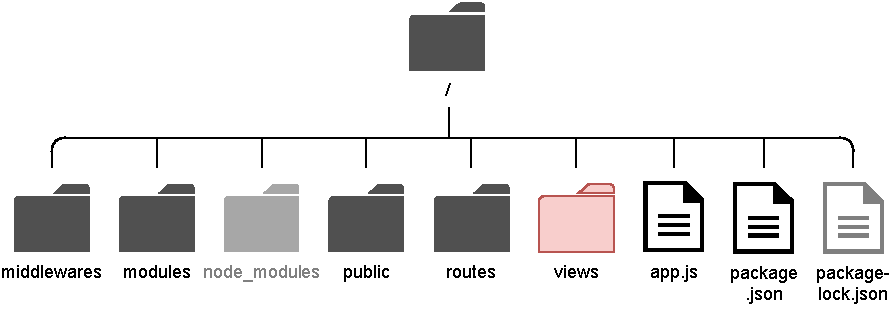
\includegraphics[width=0.75\textwidth]{includes/figures/bonus_nodejs_views.pdf}
\end{center}

\begin{defi}{Template-Engine}
    Eine \emph{Template-Engine} verarbeitet Vorlage-Dateien (\emph{Templates}) und ersetzt darin bestimmte Platzhalter durch jeweils aktuelle Inhalte.

    Im Weiteren nutzen wir das Modul \texttt{mustache-express}.
\end{defi}

\begin{example}{Views}
    \texttt{views/pokemon.tpl.html}:
    \begin{lstlisting}[language=HTML5]
        <!DOCTYPE html>
        <html>
        <head> <title> Pokemon </title> </head>
        <body>
            <table>
                <tr> 
                    <th> ID </th> 
                    <th> Name </th> 
                </tr>
                <tr> 
                    <td> ^{{id}}^ </td> 
                    <td> ^{{name}}^ </td> 
                </tr>
            </table>
        </body>
        </html>
    \end{lstlisting}

    \texttt{routes/pokemon.js}:
    \begin{lstlisting}[language=JavaScript]
        const Pokemon = require('../modules/pokemon.js') // definiert Pokemon-Klasse
        const express = require('express')
        
        module.exports = express.Router()
            .get('/', (req, res) => {
                const pokemon = Pokemon.getRand()

                res.render('pokemon.tpl.html', { // render mit json Objekt, key -> Platzhalter
                    ^'id'^: pokemon.id,
                    ^'name'^: pokemon.name 
                })
            })
    \end{lstlisting}

    \texttt{app.js}:
    \begin{lstlisting}[language=JavaScript]
        const express = require('express')
        const mustache = require('mustache-express')

        const app = express()
        const port = 3000

        /* middlewares */
        ^app.engine('html', mustache)^           // default engine, die von res.render() genutzt wird
        ^app.set('views', __dirname + '/views')^ // Ordner, in dem die engine nach html Dateien sucht

        /* routes */
        app.use('/pokemon', require('routes/pokemon.js'))
        
        app.listen(port)
    \end{lstlisting}
\end{example}